\let\negmedspace\undefined
\let\negthickspace\undefined
\documentclass[journal,12pt,twocolumn]{IEEEtran}
\usepackage{cite}
\usepackage{amsmath,amssymb,amsfonts,amsthm}
\usepackage{algorithmic}
\usepackage{graphicx}
\usepackage{textcomp}
\usepackage{xcolor}
\usepackage{txfonts}
\usepackage{listings}
\usepackage{enumitem}
\usepackage{mathtools}
\usepackage{gensymb}
\usepackage{comment}
\usepackage[breaklinks=true]{hyperref}
\usepackage{tkz-euclide}
\usepackage{listings}
\usepackage{gvv}
\def\inputGnumericTable{}
\usepackage[latin1]{inputenc}
\usepackage{color}
\usepackage{array}
\usepackage{longtable}
\usepackage{calc}
\usepackage{multirow}
\usepackage{hhline}
\usepackage{ifthen}
\usepackage{lscape}

\newtheorem{theorem}{Theorem}[section]
\newtheorem{problem}{Problem}
\newtheorem{proposition}{Proposition}[section]
\newtheorem{lemma}{Lemma}[section]
\newtheorem{corollary}[theorem]{Corollary}
\newtheorem{example}{Example}[section]
\newtheorem{definition}[problem]{Definition}
\newcommand{\BEQA}{\begin{eqnarray}}
\newcommand{\EEQA}{\end{eqnarray}}
\newcommand{\define}{\stackrel{\triangle}{=}}
\theoremstyle{remark}
\newtheorem{rem}{Remark}
\begin{document}

\bibliographystyle{IEEEtran}
\vspace{3cm}

\title{NCERT Discrete - 10.5.2.2}
\author{EE23BTECH11058 - Sindam Ananya$^{*}$% <-this % stops a space
}
\maketitle
\newpage
\bigskip

\renewcommand{\thefigure}{\theenumi}
\renewcommand{\thetable}{\theenumi}

\vspace{3cm}
\textbf{Question 10.5.2.2:} 
\begin{enumerate}
\item 30th term of the AP: 10, 7, 4, $\ldots$ is 
\item 11th term of the AP: $-3, -\frac{1}{2}, 2, \ldots$ is
\end{enumerate}
\solution
\begin{table}[h!]
    \centering
    \begin{tabular}{ | c | c | c | }
        \hline
        \textbf{Parameter}  & \textbf{value} & \textbf{Description} \\
        \hline
        \multirow{2}{*}{\begin{tabular}[c]{@{}c@{}}$x_i(0)$\\  \end{tabular}} & 10 & \multirow{2}{*}{\begin{tabular}[c]{@{}c@{}}First \\ term\end{tabular}} \\
        \cline{2-2}
        & -3 &  \\
        \hline
        \multirow{2}{*}{\begin{tabular}[c]{@{}c@{}}$d_i$ \\ \end{tabular}} & -3 & \multirow{2}{*}{\begin{tabular}[c]{@{}c@{}}Common \\ difference\end{tabular}} \\
        \cline{2-2}
          & $\frac{5}{2}$ &  \\
        \hline
        $x_1(29)$ &  ? & 30th term \\
        \hline
        $x_2(10)$ & ? & 11th term \\
        \hline
    \end{tabular}

    \caption{Input Parameters}
    \label{tab:table1}
    \end{table}\\
The $(n+1)th$ term of the AP is given by:
\begin{equation}
    x_i(n) = \sbrak{x_i(0) + n \times d_i} u(n)
    \label{eq:eq1}
\end{equation}
\begin{enumerate}
\item From the equation \eqref{eq:eq1} and the values from the table \tabref{tab:table1} :
\begin{align}
x_1(n) &= \sbrak{10 + n(-3)}u(n)\\
x_1(29) &= \sbrak{10 + (29)(-3)}(u(n))\\
&= \sbrak{10 + 29(-3)}(1)\\
&= 10+ (-87)  \\
&= -77
\end{align}
               
\begin{align}
X_1(z) = \frac{10 - 13z^{-1}}{(1-z^{-1})^2} {ROC : |z| > 1}
\end{align}

So, the 30th term of the AP is $-77$.\\
\begin{figure}[h!]
    \centering
    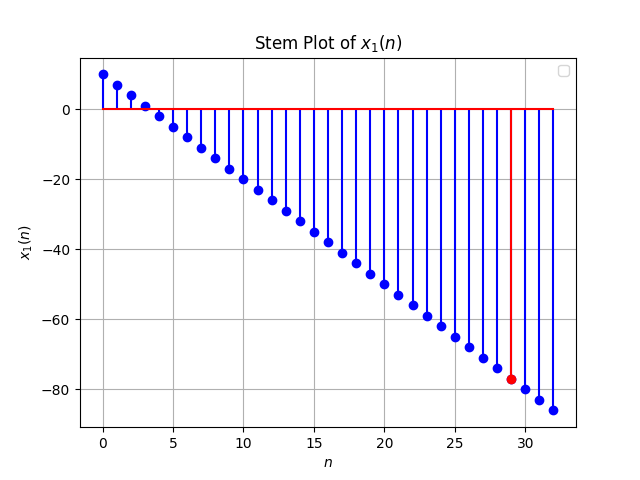
\includegraphics[width=\columnwidth]{figs/plot1.png}
    \caption{stem plot of $x_1(n)$}
    \label{fig:1}
\end{figure}

\item From the equation \eqref{eq:eq1} and the values from the table \tabref{tab:table1} :
\begin{align}
x_2(n) &= \sbrak{-3 + n\frac{5}{2}}u(n)\\
x_2(10) &= \sbrak{-3 + (10)\left(\frac{5}{2}\right)}(u(n))\\
&= \sbrak{-3 + 10(2.5)}(1)\\
& = -3 + 25 \\
&= 22
\end{align}

\begin{align}
X_2(z) = \frac{0.5z^{-1}-3}{(1-z^{-1})^2} {ROC : |z| > 1}
\end{align}


\begin{figure}[h!]
    \centering
    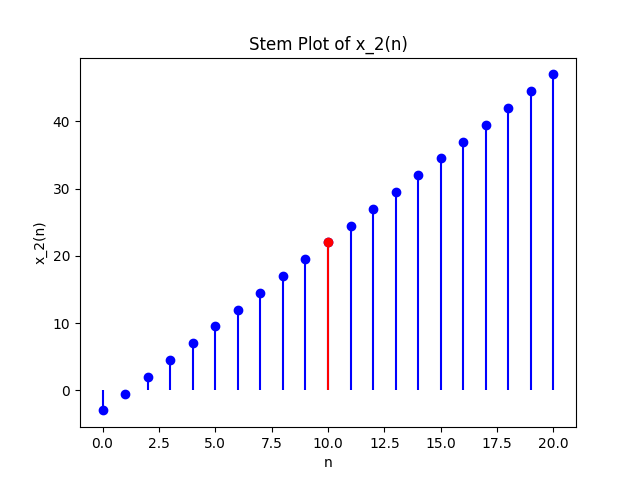
\includegraphics[width=\columnwidth]{figs/plot2.png}
    \caption{stem plot of $x_2(n)$}
    \label{fig:2}
\end{figure}
so, the 11th term of the AP is $22$.
\end{enumerate}
\end{document}
